%\documentclass[10pt,preprint]{aastex}  % for e-submission to ApJ
%\documentclass[12pt,preprint2]{aastex}  % for e-submission to ApJ - two column
\documentclass[onecolumn,iop]{emulateapj}  % this makes everything look like ApJ

\usepackage{graphicx, natbib, color, bm, hyperref, breakurl}

%%%% PUT NEW COMMANDS AND DEFINITIONS HERE %%%%
%%%% PUT NEW COMMANDS AND DEFINITIONS HERE %%%%

\newcommand{\Lmax}{\ell_{\rm max}}
\newcommand{\enzo}{{\small Enzo}}
\newcommand{\moray}{{\small Enzo+Moray}}
\newcommand{\zeus}{{\small ZEUS}}
\newcommand{\Lbox}{L_{\rm box}}
\newcommand{\Nroot}{N_{\rm root}}
\newcommand{\K}{\,\rm K}

%dcc color commands
\newcommand{\gtt}[1]{\textcolor{green}{{\tt#1}}}
\newcommand{\red}[1]{\textcolor{red}{#1}}
\newcommand{\blue}[1]{\textcolor{blue}{#1}}
\newcommand{\dcc}[1]{\textcolor{blue}{{\emph{#1}}}}

%mqk commands
\newcommand{\mqk}[1]{\textcolor{red}{mqk: #1}}
\renewcommand{\div}{\bm{\nabla} \cdot}
\newcommand{\grad}{\bm{\nabla}}
\newcommand{\curl}{\bm{\nabla} \times}

%%%% use this if you want \paragraph{} sections to be numbered.
%% \setcounter{secnumdepth}{5}

%dcc misc defs.
\def\grid{{\tt grid}}

\def\etal{{\sl et al.}}
\def\kms{{\rm km/s}}
\def\Ms{{\rm M_\odot}}
\def\nd#1{n_{ \rm #1}}
\def\k#1 {k_{{\rm #1}}}
\def\HH{H$_2$}
\def\HHp{H$_2^+$}
\def\Hp{H$^+$}
\def\Hm{H$^-$}
\def\Hep{He$^+$}
\def\Hepp{He$^{++}$}
\def\Dp{D$^+$}
\def\mHH{H_2}
\def\mH2p{H_2^+}
\def\mHp{H^+}
\def\mHm{H^-}
\def\mHep{He^+}
\def\mHepp{He^{++}}

%GB commands (overview section):
\newcommand{\myvec}[1]{\mathbf{#1}}
%\newcommand{\myvec}[1]{\vec{#1}}  %uncomment for traditional vectors
\newcommand{\rhop}{\rho^\prime}
\newcommand{\vecvp}{\myvec{v}^\prime}
\newcommand{\vecv}{\myvec{v}}
\newcommand{\vecB}{\myvec{B}}
\newcommand{\vecx}{\myvec{x}}
\newcommand{\Ep}{E^\prime}
\newcommand{\ep}{e^\prime}
\newcommand{\phip}{\phi^\prime}
\newcommand{\pp}{p^\prime}
\newcommand{\vecr}{\myvec{r}}
\newcommand{\rhob}{\rho}
\newcommand{\vecvb}{\vecv}
\newcommand{\Mach}{\mathcal{M}}
\newcommand{\fcond}{\myvec{F}_{\rm cond}}
\newcommand{\minmod}[2]{{\rm minmod} \left({#1},{#2} \right) }

%JHW commands
\newcommand{\cubecm}{\ifmmode{{\rm cm^{-3}}}\else{cm$^{-3}$}\fi}
\newcommand\unit[1]{\; \textrm{#1}}
\newcommand{\mh}{m_{\rm H}}

%SWS commands
\newcommand\abs[1]{\left|#1\right|}



\citestyle{aa}  % correct formatting for ApJ style files

\begin{document}

\title{Phd: Phython Hydro-Dynamics Code for Astrophysics}
\author{Ricardo Fernandez\altaffilmark{1}}
\author{Greg L. Bryan\altaffilmark{1,2}}

\altaffiltext{1}{Columbia University, Department of Astronomy, New York, NY, 10025, USA}
\altaffiltext{2}{Center for Computational Astrophysics, Flatiron Institute, 162 Fifth Avenue, New York, NY 10010}

\begin{abstract}
This paper describes the open-source code \enzo, which uses
block-structured adaptive mesh refinement to provide high spatial and
temporal resolution for modeling astrophysical fluid flows.
\end{abstract}

\keywords{methods: numerical --- hydrodynamics}

\maketitle

% Section: introduction
\section{Introduction}
\label{sec.intro}

The use of numerical simulations for modeling astrophysical compressible 
gas have steadily grown through the rise of computing power and decrease
in price of hardware. Astrophysical problems poses its unique set of challenges
manifesting throught its high spatial and temporal dynamic ranges. Progress
has been made over the years by the development of algorithms that leverage
computing resources to the problem at hand. The two most notable numerical methods 
are Langrangian and Eulerian schemes. A popular example of Langrangian scheme
is the smoothed particle hydrodyanmics developed by ... 

In this scheme
talk  about sph strengths and weakness

talk about eulerian

talk

For example adaptive mesh refinement
allows for dynamic addition of computing grids. This feature allows computing
resources to adaptively  

\subsection{Motivation for ALE}
\label{sec.motivation_ale}

Due to the high spatial and temporal dynamical ranges involved,

\subsection{Motivation for Python}
\label{sec.motivation_python}

Due to the high spatial and temporal dynamical ranges involved,

\subsection{Design Philosophy}
\label{sec.design_philosophy}

Due to the high spatial and temporal dynamical ranges involved,


% Section: numerical methods
\section{Physics and Algorithms}
\subsection{Physical Equations}
\label{sec.physical.eq}
The spatial and temporal evolution of a compressible fluid is governed by the
Euler equations. The Euler equations are a set of hyperbolic conservation laws
governing the density $\rho$, velocity $\mathbf{v}$, and total specific energy
$E$ (specific kinetic energy $\frac{1}{2}\rho \mathbf{v}^2$ plus specific internal
energy $u$). These quantities $\mathbf{U}$ and their respective fluxes
$\mathbf{F}(\mathbf{U})$, defined through the Euler equations, are conveniently
expressed in vector form as
%
\begin{equation}
    \mathbf{U} =
    \left(
    \begin{array}{c}
        \rho \\
        \mathbf{v} \\
        \rho e \\
    \end{array} \right),
    \quad
    \mathbf{F}(\mathbf{U}) =
    \left(
    \begin{array}{c}
        \rho\mathbf{v} \\
        \rho\mathbf{v}\mathbf{v}^T + P \\
        \rho e\mathbf{v} + P\mathbf{v} \\
    \end{array}
    \right),
\end{equation}
%
where P is the pressure. In this notation the Euler equations can be expressed
in the form
%
\begin{equation}
    \label{eq.euler}
    \frac{\partial \mathbf{U}}{\partial t} + \div \mathbf{F} = 0.
\end{equation}
%
As stated the system of equations are not closed; there are more variables then
equations. Thus, a constraint is needed and is supplied by the equation of state, which is typically given by the ideal gas relation
%
\begin{equation}
    P = \rho(\gamma - 1)u,
\end{equation}
%
where $\gamma$ is the ratio of specific heats.

These equations can be solved by the finite-volume approach, which is a
discretization of the domain into finite sized disjoint cells and evolves their
spatial averaged $\mathbf{U}$ values. Specifically, applying equation
(\ref{eq.euler}) to every cell $i$ with volume $V_i$ and performing Gauss'
theorem to convert the volume integral to a surface integral results in
%
\begin{equation}
    \label{eq.euler.int}
    \frac{d\mathbf{Q}_i}{dt} =
    -\sum_{j}\int\mathbf{F}_{ij}(\mathbf{U})\cdot\mathbf{A}_{ij},
\end{equation}
%
where $\mathbf{A}_{ij}$ is the cell's surface area normal and $\mathbf{Q}_i$
is the volume integral of $\mathbf{U}_i$,
%
\begin{equation}
	\mathbf{Q}_i =
    \left(
    \begin{array}{c}
    	m_i \\
        \mathbf{p}_i \\
        E_i
     \end{array}
     \right) = \int_{V_i}\mathbf{U}_i dV,
\end{equation}
where $m_i$, $\mathbf{p}_i$ and $E_i$ are cell's total mass, momentum, and
energy, respectively. Here, an assumption is taken that the cell's volume
is a polyhedron such that the surface integral can become a sum over all
polygon faces. Additionally, time is discretized leading to a finite difference
update of the cell's quantities given by
%
\begin{equation}
    \label{eq.flux.update}
    \mathbf{Q}_i^{n+1} = \mathbf{Q}_i^n - \Delta t\sum_j
    \mathbf{\hat{F}}_{ij}^{n+1/2} A_{ij}.
\end{equation}
%
In this expression, the flux $\mathbf{\hat{F}}^{n+1/2}$ is taken to be a time
average and is constant across the cell face. To be able to use equation
\ref{eq.flux.update} we must make estimates of
$\mathbf{\hat{F}}^{n+1/2}$ and $A_{ij}$ to the proper order of accuracy. Sections \ref{sec.riemann} and
\ref{sec.tessellation}, respectively, will go into detail on how these quantities are
estimated.

\subsection{Tessellation}
\label{sec.tessellation}
As stated in Section \ref{sec.physical.eq}, the Euler equations, as written in
(\ref{eq.flux.update}), assume that the cells are in the form of polyhedrons.
There are many ways of partitioning space that meet this criteria but for this
paper we will restrict our attention to the Voronoi tessellation. The Voronoi
tessellation partitions the space into a set of disjoint polyhedrons for a
given set of points. The set of points are called mesh generators and for each
generator there is a corresponding region consisting of all points that are closer
to that generator than any other. Thus, for each mesh generating pair there
lies a polygon that is equidistant. This geometric property will be exploited
in several ways. For the rest of this paper we will refer to the polyhedra
associated with the mesh generator as a cell and the polygons making up the
polyhedra as faces.

The creation of the Voronoi tessellation can be performed by first constructing
the Delaunay triangulation. The Delaunay tessellation is the dual graph of the
Voronoi tessellation and is defined as the triangulation of points such that
no point in the set lies inside the circumcircle of any of the triangles, in
2d. In 3d the triangles become tetrahedron but the same definition applies.
Remaining in 2d for simplicity, the points are the vertices of the triangles.
The dual aspect refers to the fact that each triangle edge corresponds to a
Voronoi face and each Voronoi vertex corresponds to the center of the
circumcirlce of the triangle. 

\subsection{Fluid Update}
\subsubsection{Reconstruction}
% Need some introductory text
To solve the Riemann problem, primitive values are needed at the face. As a first
choice, cell center values can be used. Although for more accurate results a 
method is needed to extrapolate the cell center values to the center of mass of 
the face. At first order, in space and time, can be constructed by Taylor-series 
expanding the primitive values
%
\begin{equation}
	\label{eq.taylor}
	\mathbf{W}' = \mathbf{W} + \frac{\partial\mathbf{W}}{\partial\mathbf{r}}
    	(\mathbf{f}-\mathbf{s}_i) + \frac{\partial\mathbf{W}}
        {\partial t}{\Delta t}.
\end{equation}
%
The expansion has two unknowns, the spatial derivative
$\frac{\partial\mathbf{W}}{\partial \mathbf{r}}$ and the time derivative
$\frac{\partial\mathbf{W}}{\partial t}$. However, both derivatives
are related through the Euler equations in primitive form
%
\begin{equation}
    \frac{\partial\mathbf{W}}{\partial t}  + \mathbf{A}
    	(\mathbf{W})\frac{\partial\mathbf{W}}{\partial\mathbf{r}} = 0,
    \quad
    \mathbf{A}(\mathbf{W}) =
    \left(
    \begin{array}{ccc}
        \mathbf{v} & \rho & 0 \\
        0 & \mathbf{v} & 1/\rho \\
        0 & \gamma P & \mathbf{v}
    \end{array}
    \right).
\end{equation}
%
Thus, only the spatial derivatives need to be calculated. For the
calculation we follow the method presented in (Springel), which is
summarized below. Given a cell $i$ the components of 
$\frac{\partial\mathbf{W}}{\partial \mathbf{r}}$, which are gradients
of the primitive variables, are given by
%
\begin{equation}
	\nabla\phi_i = \frac{1}{V_i}\sum_{j}A_{ij}
    	\left(\left[\phi_i - \phi_j\right]\right) -
        \frac{\phi_i + \phi_j}{2}
        \frac{\mathbf{r}_{ij}}{r_{ij}}.
\end{equation}
%
The sum is over all neighbors $j$ of particle $i$, $\phi_i$ and
$\phi_j$ are the scalar field values at each cell center respectively,
$\mathbf{r}_{ij} = \mathbf{r}_i - \mathbf{r}_j$ is the separation vector
with magnitude $r_{ij} =|\mathbf{r}_{ij}|$. As constructed, the gradients
are second order in space for smooth flows. However, in the presence of
shocks, numerical instabilities may arise and therefore the reconstruction
must be reduced. To deal with this a slope limiter is used. We employ two
limiters. The first one is the method used by AREPO and begins with
the calculation of
%
\begin{equation}
		\psi_{ij} = \left\{
  		\begin{array}{@{}ll@{}}
    		(\phi_i^{max} - \phi_i)/\Delta \phi &
            	\text{for}\ \Delta\phi_{ij} > 0 \\
            (\phi_i^{min} - \phi_i)/\Delta \phi &
            	\text{for}\ \Delta\phi_{ij} < 0 \\
            1 & \text{for}\ \Delta\phi_{ij} = 0,
  		\end{array}\right.
\end{equation}
%
where $\phi_i^{max} =$ max$(\phi_j)$ and $\phi_i^{min} =$ min$(\phi_j)$ are
the maximum/minimum values across all neighbors of $i$ and
$\Delta\phi_{ij} = \nabla \phi_i \cdot (\mathbf{f}_{ij} - \mathbf{s}_i)$. Then 
the minimum of all $\psi_{ij}$s, associated with each primitive field, is found 
producing a single scalar value
%
\begin{equation}
	\alpha_i = min(1, \psi_{ij})
\end{equation}
%
 that is used to limit the gradient
%
\begin{equation}
	\nabla \phi_i' = \alpha_i \nabla \phi_i
\end{equation}

\subsubsection{Riemann Solve}
\label{sec.riemann}
The Riemann problem consist of two constant states separated by an interface.
The solution to this problem is the formation of three waves emanating from the
interface. These waves are associated with the eigenvalues of the Euler equations
and each carry a jump in the characteristic variables. The goal of the Riemann
solver is to estimate these nonlinear waves and construct the fluxes at the
interface. Four purposes, we have elected to use the HLL, HLLC, and Exact Riemann
solvers. 
 
The HLL solver ignores the contact in solving the Riemann problem. In this case
only two waves are considered.

\subsection{Grid Motion}
As currently constructed the method outlined in solving the Euler equations are 
for static meshes only. In our case we allow the mesh to move, meaning the mesh
generators are given some velocity $\mathbf{w}_i$. Thus, equation \ref{eq.euler}
must be augmented to account for an advection term produced by the movement
of the face. The updated Euler equations become
%
\begin{equation}
	\label{eq.euler.moving}
    \mathbf{F}_m(\mathbf{U}) = \mathbf{F}_s(\mathbf{U})
    	- \mathbf{U}\mathbf{w}^T =
    \left(
    \begin{array}{c}
        \rho\mathbf{v} \\
        \rho\mathbf{v}\mathbf{v}^T + P \\
        \rho e\mathbf{v} + P\mathbf{v} \\
    \end{array}
    \right) -
    \left(
    \begin{array}{c}
        \rho\mathbf{w} \\
        \rho\mathbf{v}\mathbf{w}^T \\
        \rho e\mathbf{w} \\
    \end{array}
    \right).
\end{equation}
%
In practice equation  is not used because of its unstable
numerical behavior (Parkmor). The equation can become numerical stable by
solving the fluxes in the rest frame of the face. At the face the conserved 
variables and fluxes become
%
\begin{equation}
	\mathbf{U}' =
    \left(
    \begin{array}{c}
        \rho \\
        \rho(\mathbf{v-w}) \\
        \rho e' \\
    \end{array} \right),
    \quad
   	\mathbf{F}'(\mathbf{U}') = 
    \left(
    \begin{array}{c}
        \rho(\mathbf{v-w}) \\
        \rho(\mathbf{v-w})(\mathbf{v-w})^T + P \\
        \rho e'(\mathbf{v-w}) + P(\mathbf{v-w}) \\
    \end{array}\right) =
    \left(
        \begin{array}{c}
        F_\rho' \\
        F_\mathbf{v}' \\
        F_e' \\
    \end{array}
    \right).
\end{equation}
%
Notice $\rho$ and $P$ remain unchanged however the $e$ transform to
$e' = e -\frac{1}{2}\mathbf{v}^2 + \frac{1}{2}(\mathbf{v-w})^2$. Now
the fluxes need to be transformed back to the lab frame
%
\begin{equation}
	\label{eq.euler.face}
    \mathbf{F}_m(\mathbf{U}) = \mathbf{F}_s(\mathbf{U})
    	- \mathbf{U}\mathbf{w}^T = \mathbf{F}'(\mathbf{U}') +
    \left(
    \begin{array}{c}
        0 \\
        \rho\mathbf{w}(\mathbf{v-w})^T \\
        \rho(\mathbf{vw})(\mathbf{v-w}) -\frac{\rho}{2}
        	\mathbf{w}^2(\mathbf{v-w}) + p\mathbf{w} \\
    \end{array}
    \right),
\end{equation}
%
where the terms have been picked to make equation \ref{eq.euler.face} consistent with
equation \ref{eq.euler.moving}. This equation can be restated in terms of the rest
frame fluxes,
%
\begin{equation}
	\label{eq.final.euler}
    \mathbf{F}_m(\mathbf{U}) = \mathbf{F}_s(\mathbf{U})
    	- \mathbf{U}\mathbf{w}^T = 
    \left(
    \begin{array}{c}
        F_\rho' \\
        F_\mathbf{v}' + \mathbf{w} F_\mathbf{v}'^T \\
        \mathbf{w}F_\mathbf{v}' + \frac{1}{2}F_\rho' \mathbf{w}^2
    \end{array}
    \right).
\end{equation}
%
Thus, after solving the riemann problem in the rest frame of the face the fluxes
can be easily transformed back into the lab frame. Finally, to make use of equation
\ref{eq.final.euler} with \ref{eq.taylor} the primitive variables need to transformed
by the following
%
\begin{equation}
    \mathbf{W}' = \mathbf{W} - 
    \left(
    \begin{array}{c}
        0 \\
        \mathbf{w} \\
        0 \\
    \end{array}
    \right).
\end{equation}
%
This ensures that the correct values are used in the riemann solver.

\subsubsection{Time Integration}
The time integration using equation \ref{eq.euler.int} with \ref{eq.taylor} is
a form of the MUSCL-Hancock scheme. For static meshes, the scheme is second
order accurate in space and time. However, letting the mesh move introduces
inaccuracies due to ignoring the effect of the mesh deformation during a time 
step $\Delta t$. This can be corrected by adopting a Runge-Kutta type scheme, that
uses information from the beginning and the end of a time step instead of mid
point estimations. Specifically, we employ the method outlined by (Pakmor)
which updates the conservative variables by the following
\begin{equation}
	\begin{array}{rcl}
		\mathbf{W}_i' & = & \mathbf{W}_i^n + 
        	\Delta t\frac{\partial\mathbf{W}}{\partial t}, \\
        \mathbf{r}' & = & \mathbf{r}^n + \Delta t\mathbf{w}^n, \\
        \mathbf{Q}_i^{n+1} & = & \mathbf{Q}_i^n -
        	\frac{\Delta t}{2}\left(\sum_j A_{ij}^n\mathbf{\hat{F}}_{ij}^n
            (\mathbf{W}^n) + \sum_j A_{ij}'\mathbf{\hat{F}}_{ij}'
            (\mathbf{W}')\right), \\
        \mathbf{r}^{n+1} & = & \mathbf{r}'.
    \end{array}
\end{equation}
Here we are taking an average of the fluxes from the beginning and the end
of the time step. The flux at the beginning of the time step is constructed
with the current state of the mesh with the primitive values extrapolated to
the face. Then the mesh generators move to their final position
and the mesh is reconstructed. A new flux is constructed with new geometric
quantities, however, the primitive values have been extrapolated in time from
the beginning of the time step. At first glance, it seems that the mesh has
to be constructed twice per time step. However, the generator velocity is
treated constant throughout the time step resulting the final mesh to be equal to
the beginning mesh of the next time step. Thus, the mesh need only to
be constructed once per time step while the fluxes have to be calculated
twice per time step. This method is not truly a Runge-Kutta scheme because
of the time extrapolation but more a mixture of Runge-Kutta and MUSCL-Hancook
scheme that has been shown to be second order accurate in space and time.

\subsubsection{Regularization}
Allowing the mesh generators to move with the local fluid velocity 
$\mathbf{w}_i$ can lead to cells that are elongated or mesh generators close to 
given face. This results, to an unstable evolution of the cells because their 
faces can move rapidly relative to the generator velocity (Duffell). To 
counteract this issue (Springel) proposed a correction term that would steer the 
generator towards its center of mass. This effectively causing the cell to 
become rounder, thus mitigating the issue. The correction term is defined as
%
\begin{equation}
	\mathbf{w}_i' = \mathbf{w}_i + \chi\left\{
  		\begin{array}{@{}ll@{}}
    		0, & \text{for}\ d_i/(\eta R_i) < 0.9 \\
    		c_i\frac{\mathbf{s}_i - \mathbf{r}_i}{d_i}
            	\frac{d_i-0.9\eta R_i}{0.2\eta R_i}, 
            	& \text{for}\ 0.9 \leq d_i/(\eta R_i) < 1.1 \\
            c_i\frac{\mathbf{s}_i - \mathbf{r}_i}{d_i},
               	& \text{for}\ 1.1 \leq (d_i)/(\eta R_i).
  		\end{array}\right.
\end{equation}
%
Here $R_i$ is the effective radius of the cell, $(V_i/\pi)^{1/2}$ for 2d and
$(3V_i/4\pi)^{1/3}$ for 3d, $d_i$ is the distance between the generators
position $\mathbf{r}_i$ and center of mass $\mathbf{s}_i$, $c_i$ is the local sound speed. $\chi$ and $\eta$ are tunning parameters which are typically set 
to 0.25 and 1.0, respectively.

\subsection{External Boundary Conditions}
For each simulation a boundary condition must be defined. At this moment, only
reflection and periodic boundaries are implemented. Our domains are restricted to
rectangular domains with arbitrary aspect ratios. The implementation of both
boundaries make use of ghost particles. These ghost particles are created during
the mesh construction and carry all particle information to participate in the 
integration step. From the simulation perspective, they are treated as real particles,
however, after a time step all ghost particles are discarded and new ghost particles
are formed with the relevant updated particle information.

\subsubsection{Periodic}
Periodic boundaries are formed by examining the circumcirlce of each real particle
in the tessellation. If this value intersects the domain boundary the particle is
flagged for ghost construction. The flagged particle is then shifted periodically in
all dimensions including corner cases and tested for boundary intersection. If 
intersection occurs a ghost particle is formed from the particle but with the
appropriate position data.

\subsubsection{Reflecting}
The reflection boundary parallels the periodic case with exception that particles
are not periodically shifted. Instead, the flagged particle is mirrored across the
minimum and maximum of each boundary dimension. If intersection occurs, again, a ghost
particle is formed, however, the sign of the normal velocity component is flipped.
This ensures that the mass flux vanishes on the surface of the boundary.

\subsection{Gravity}
In the presence of gravity the Euler equations \ref{eq.euler} are modified by
a source term
%
\begin{equation}
    \frac{\partial \mathbf{U}}{\partial t} + \div \mathbf{F} =\left( 
    \begin{array}{c}
    	0 \\
        -\rho\nabla\mathbf{\Phi} \\
        -\rho\mathbf{v}\nabla\mathbf{\Phi}
    \end{array}\right).
\end{equation}
%
Note that the gravitational potential $\mathbf{\Phi}$ only affects the
momentum and energy. The source of the potential can be prescribed by
an external source or by the self gravity of the gas. In the latter case
the potential is given by Poisson's equation
%
\begin{equation}
	\nabla^2\mathbf{\Phi} = 4\pi G\rho
\end{equation}
For the moment assume that $\mathbf{\Phi}$ is given. Then the equations
\ref{eq.taylor} and \ref{eq.euler.int} can be easily supplemented to
include the gravitational force. First, the time derivatives in the
reconstruction equation are replaced by
%
\begin{equation}
    \frac{\partial\mathbf{W}}{\partial t}  + \mathbf{A}
    	\left(\mathbf{W}\right)\frac{\partial\mathbf{W}}{\partial\mathbf{r}}
        = \left(
        	\begin{array}{c}
            0 \\
            -\nabla\mathbf{\Phi} \\
            0
            \end{array}
         \right),
\end{equation}
%
In this case the time extrapolated variables include a gravitational
component. Second, the momentum and energy is updated during the flux update
%
\begin{equation}
	\begin{array}{rcl}
        \Delta\mathbf{p}_i & = &
        	\frac{\Delta t}{2}\left(\sum_j A_{ij}^n\mathbf{\hat{F}}_{ij,\mathbf{p}}^n
            (\mathbf{W}^n) + \sum_j A_{ij}'\mathbf{\hat{F}}_{ij,\mathbf{p}}'
            (\mathbf{W}')\right) - \frac{1}{2}\Delta t\left( 
        	m_i\nabla_i\mathbf{\Phi} + m_i'\nabla_i\mathbf{\Phi}'\right)\\
        \Delta E_i & = &
        	\frac{\Delta t}{2}\left(\sum_j A_{ij}^n\mathbf{\hat{F}}_{ij,E}^n
            (\mathbf{W}^n) + \sum_j A_{ij}'\mathbf{\hat{F}}_{ij,E}'
            (\mathbf{W}')\right) - \frac{1}{2}\Delta t\left( 
        	m_i\mathbf{v}_i\nabla_i\mathbf{\Phi} +
            m_i'\mathbf{v}_i'\nabla_i\mathbf{\Phi}'\right)\\
    \end{array}
\end{equation}
%
\subsubsection{Constant}
\subsubsection{Tree}

\subsection{Parallelism}
\subsubsection{Partitioning}
For domain decomposition we follow the approach of (Springel) and use
a space filling curve. Here every particle position is mapped onto a
1D line. The line is decomposed into a number or roughly equal pieces.
The number of segments is equal to the number of processor for the
give run.

In practice, for each particle a Peano-Hilbert key is computed. The key

\subsubsection{Ghost particle copying}
For ghost particle we make a further distinction, interior and exterior ghost particles.
Interior ghost particles are only used in parallel simulations while exterior ghost
particles are associated with the boundary conditions of the simulation. In the following
section we will go into the details on how the DomainManager creates ghost particles
and transfers data.


% Section: code overview
\section{Code Design}
\subsection{Overall Class Design Considerations}
\subsubsection{Field Registration}
\subsubsection{Class Registration}

\subsection{Particle Data Structures}
\subsubsection{Carray}
In choosing the underlying data structure several considerations where taken. First the
data had to be accessible in python and in C. Second the data structure had to
accommodate several data types. For this reason we choose a data structure that mimics
numpy arrays, in the sense that raw data is allocated in C and interface exist that
manipulates the data in either C or python. With this approach a decision had to be
made in the form of the raw data. Two choices where considered, either the data would
be held in structs or arrays. The benefit of structs would allow subfields of the data
be compact and allow easy implementations of passing and receiving data from other
processors in parallel runs. Further numpy has an interface, that treats
arrays of structs as record numpy arrays. However, this form was abandoned early on
as the sub-fields would have to be hard coded and would not allow the creation of
dynamic fields at run time. With this consideration, the raw data was chosen to be
c arrays. 

The exact implementation was taken from pysph code. The class is called Carray and
can be initialized in Python or Cython. The interface closely resembles the list
class of c++, in allowing indexing and memory management. Further, Carrays can return
a numpy array, allowing the user to use all numpy functional (i.e. slicing and facny indexing). 
Below is a simple example using a Carray.
\begin{lstlisting}
import phd

x = phd.DoubleArray(10)
for i range(len(x)):
	x[i] = i**2
    
x.append(3.21)
x.resize(5)

xnp = x.get_npy_array()
xnp[:] = np.arange(x.length)
\end{lstlisting}
In this example a Carray is created with 10 doubles, then assigned values by indexing. Notice
that the length of the Carray can be found either by the len function or the length
attribute. The Carray then has a value appended to it followd by resizing the Carray to a length
of 5. Finally, the get npy array is called returing a numpy array which allows the use of slicing.

\subsubsection{CarrayContainer}
The use of Carrays allow to easily manipulate arrays of certain type of data. However, there are
many circumstances for the need of a collection of Carrays. For example the x, y, and z position
of a particle or the center of mass and moments of a node in the gravitational tree. Therefore,
another data structre has been implemented to facilitate the use of collection of Carrays. The data
structure is called a CarrayContainer and like the Carray it has many methods to manipulate the
underlying data. The CarrayContainer in some aspects mimics a python dicitionary in the sense
that each carray can be retrieved by a string key.
\begin{lstlisting}
import phd
import numpy as np

carrys = {"x": "double", "x", "double"}

ca_con = phd.CarrayContainer(10, carrays)
size = ca_con.get_carray_size()
ca_con["x"][:] = np.random.rand(size)
ca_con["y"][:] = np.random.rand(size)

ca_con2 = phd.CarrayContainer(5, carrays)
size = ca_con.get_carray_size()
ca_con["x"][:] = np.random.rand(size)
ca_con["y"][:] = np.random.rand(size)

ca_con.append(ca_con2)
ca_con.remove(np.array([1, 3, 9])
\end{lstlisting}
Most of the routines of Carrays have been extented to CarrayConatiner to operate on
all Carrays in the Container. Further the container has routines to subet, remove, paste
and add values to certain elements.

\subsection{Simulation Class}
\subsubsection{Serialization of classes and parameters}

\subsection{Mesh Class}
\subsubsection{Tessellation}
\subsubsection{Grid Motion}
\subsubsection{Flux Update}

\subsection{Integrator Class}

\subsection{Hydro Class}
\subsubsection{Reconstruction}
\subsubsection{Riemann Solver}

\subsection{General Source Terms}
\subsubsection{Gravity}

\subsection{Readers/Writers}
\subsubsection{HDF5}

\subsection{Outputters and Finishers}
\subsubsection{Design API}
\subsubsection{Examples}

\subsection{Load Balance}

\subsection{Equation of State}

\subsection{Domain Manager}
\subsubsection{Internal Boundary Particle Sharing}
\subsubsection{Particle Motion}
\subsubsection{Boundary Condition}

\subsection{Logging}

\subsection{Units}

\subsection{Profiling}


% Section: code tests
\section{Tests}
\subsection{Unit Tests}

\subsection{Hydro Tests}
\subsection{Linear Wave}
Sound waves provide the mechanism to transport disturbances in a fluid. An
elementary test problem is the ability maintain wave propagation of small
disturbances . Given a fluid in equilibrium with constant density $\rho_0$,
pressure $p_0$ and zero velocity $\mathbf{v}=0$ with perturbations of the form
\begin{equation}
	\begin{array}{rcl}
		\rho & = & \rho_0 + \delta\rho(x,t) \\
   		 p & = & p_0 + \delta p(x,t) \\
    	\mathbf{v} & = & \delta\mathbf{v}(x,t),
    \end{array}
\end{equation}
and maintaining terms to first order in the Euler equations produce the wave
equation for each variable with a wave propagation speed equal to the fluids sound speed 
$c_s$ suffice the perturbations are small. Thus, setting a small disturbance will propagate 
with a finite velocity maintaining 
its form.

We set up a 2d box of unit length with constant $\rho_0=1.0$, $p_0=3/5$, $\mathbf{v}=0$,
and $\gamma=5/3$ with periodic boundary conditions. A sinusoidal wave in the x direction of 
the form $\delta\rho(x,t) = Asin(kx + wt)$ with $k=w=2\pi$ and $A=10^{-6}$ is added at time 
$t=0$. The remaining disturbances can be specified through $\delta\rho$ by the following
\begin{equation}
	\begin{array}{rcl}
        \delta \mathbf{v}(x,0) & = & \left(\frac{w}{k}\right)\delta
        	\rho(x,0)/\rho_0\mathbf{\hat{x}}\\
        \delta p(x,0) & = & \left(\frac{w}{k}\right)^2\delta\rho(x,0).
    \end{array}
\end{equation}
The values chosen produce waves traveling rightward with a velocity of 1. The simulation is
ran for 1 time unit such that the waves return to its initial position at time $t=0$. 
Moreover, we study the convergence behavior by comparing the final state of the density to 
the initial density by computing the $L1$ norm,
\begin{equation}
	L1 = \frac{1}{N^2}\sum_i \left| \rho_i - \rho(x_i) \right|,
\end{equation}
where $\rho_i$ is final density at position $x_i$ and $\rho(x_i)$ is the density at t=0
at position $x_i$ and $N$ is the number of cells per dimension. Five simulations where ran
with varying resolution $N=10, 20, 40, 80, 160$. The initial particles where laid out in a
Cartesian grid and the mesh was allowed to move with the fluid velocity. All simulations
where performed with linear reconstruction and the HLLC solver.
\begin{figure}
    \begin{center}
        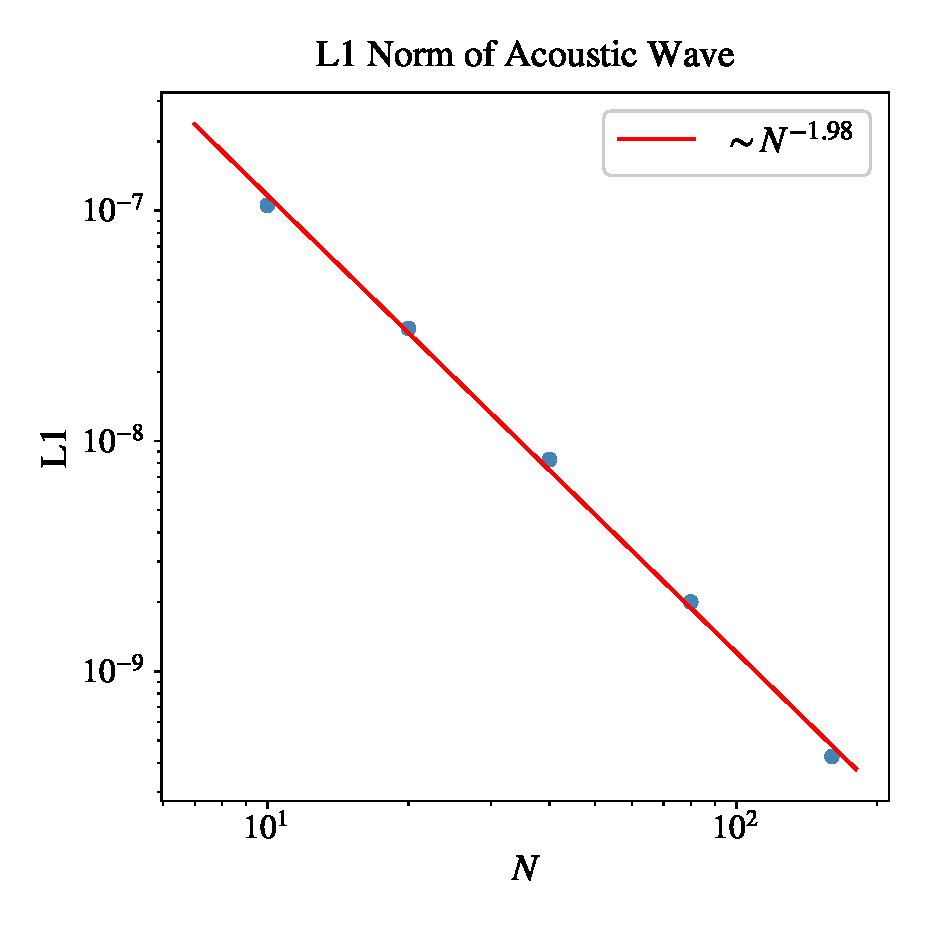
\includegraphics[width=0.4\textwidth]{figures/acoustic-wave-l1.eps}
        \caption{L1 norm of acoustic wave problem in 2d. Blue points are results
        of simulation from different resolutions overlayed by a linear fit showing
        the convergence is approximately second order.}
        \label{fig.acoustic}
    \end{center}
\end{figure}


\subsubsection{Sod Shock Tube}
\subsubsection{Sedov}
\subsubsection{Kelvin Helmholtz}

\subsection{Gravity Tests}
\subsubsection{Rayleigh Taylor}
\subsubsection{Two body}
\subsubsection{Evrard Collapse}

\subsection{Chemistry Tests}
\subsubsection{Uniform Cooling}


% Section: conclusions
%%%%%%%%%%%%%%%%%%%%%%%%%%%%%%%%%%%%%%%%%%%%%%%%%%%%%%%%%%%%%%%%%%%%%%%%%%%%%%
\section{Conclusions}
\label{sec.conclusions}

In this paper, we have presented the algorithms underlying \enzo, an
open-source adaptive mesh refinement code designed for
self-gravitating compressible fluid dynamics, including the effects of
magnetic fields, radiation transport, and a variety of microphysical
and subgrid processes.  In addition, we have described the \enzo\ code
development process, have shown the outputs of a set of representative
test problems, and have provided information about \enzo's performance
and parallel scaling on recent supercomputing platforms.  The \enzo\
code, its test suite, and all of the scripts used to generate plots
and figures for this paper are open source and are available at the
\enzo\ website, \url{http://enzo-project.org}.  Furthermore, the
\texttt{yt} toolkit, which is designed to analyze \enzo\ data (as well
as data from a wide variety of other simulation tools), can be found
at its website, \url{http://yt-project.org}.  Both of these codes have
active user and developer communities, extensive documentation and
user support, and strong mechanisms for users to contribute their
changes and fixes to the codebase.

The developers of the \enzo\ code are currently working on several
projects that will extend the functionality, scalability, or overall
performance of the code in the near future.  Projects that will appear
in forthcoming releases of the \enzo\ code include:

\begin{itemize}
\item The creation of a hybrid-parallel version of \enzo, combining
MPI for communication between nodes of a supercomputer and OpenMP for
thread-based parallelism within a node.  This will reduce on-node
memory usage and improve overall scaling behavior.
\item The restructuring of \enzo's treatment of particles to
accommodate a wider range of ``active'' particles that can easily
interact with each other and with multiple grids, and include sink,
source, and particle creation, destruction, splitting, and merging
functionality.
\item A new HYPRE-based AMR gravity solver that is faster, more
accurate, and more scalable than the current multigrid solver.
\item New infrastructure for problem initialization, enabling users to
more quickly and easily create new types of simulations.
\end{itemize}

With the continual rapid development of computer hardware, it makes
sense to not only review \enzo's current capabilities, but to look
toward its future development in view of predicted technological
trends. These trends in supercomputing hardware suggest that
substantial modifications to \enzo's core infrastructure, and very
possibly some of the core algorithms, will be required. More
specifically, the progression involves the usage of specialized
large-core-count, vectorized computing units such as graphics
processing units or chips like the Intel Xeon Phi, as well as
precipitously decreasing amounts of RAM per computing core.  The
former trend means that the amount of processing power per compute
node will continue to increase, likely much faster than the bandwidth
between nodes, and will require tremendous reduction in inter-node
(and possibly inter-CPU) communication in order to maintain code
scalability.  Also, much of the current code will need to be rewritten
to take advantage of the vector nature of these CPUs, making
assumptions that are quite unlike those made in much of the current
codebase.  The latter trend means that duplication of data -- for
example, the grid hierarchy -- must be effectively eliminated to save
memory, and all inter-core and inter-node communication must be
carefully thought through to minimize the amount of data moved.  An
additional challenge as one goes to core counts in the tens to
hundreds of millions (or more) is that the reliability of individual
computing elements will become much more of an issue, requiring
robustness to hardware failure to be built into the code at some
level.  Furthermore, we are nearing the physical limits of transistor
speed and interconnect latency~\citep{feynman1999feynman}, meaning
that simple hardware improvements will not make these challenges
disappear, and careful thought (and the rewriting of a great deal of
code) must take place!  These challenges are not unique to the \enzo\
code, and in fact are faced by effectively all applications that wish
to take advantage of new computational architectures. We therefore
anticipate that \enzo\ (or a code that has the capabilities of \enzo,
from a user's point of view) will continue to be usable at the largest
scales on such machines.

  

\acknowledgments


\appendix
\section{Interpolation methods}
\label{app:interpolation}

In this appendix, we provide details for the various interpolation
methods available in the code.  We assume throughout that we are
dealing with Cartesian coordinates and cells of equal sizes, although
we allow for an arbitrary refinement factor $r$ between cells at
different levels.

\vspace{0.5cm}\noindent
{\bf SecondOrderA} 

This interpolation algorithm is generally second-order, but has
monotonicity constraints as described below.
In one dimension, we define the parent values as $Q_{-1}$, $Q_0$, and
$Q_{+1}$, where the central parent cell has a left edge at $x_0$ and
width $\Delta x$. We first linearly interpolate the parent values to
the cell edges: $Q_{-1/2} = (Q_0 + Q_{-1})/2$, and similarly for
$Q_{1/2} = (Q_0 + Q_1)/2$, and then compute a monotonic slope: $\Delta
Q_0 = \minmod{Q_{1/2} - Q_0}{Q_0 - Q_{-1/2}}$ where

\begin{equation}
\minmod{a}{b} = \left\{ \begin{array}{ll}
0 & {\rm if} \quad ab < 0 \\
\min{ \left( | a |, | b | \right) } {\rm sign} (a) & {\rm otherwise}
\end{array}\right.
\end{equation}

This slope is then used to compute the interpolated subgrid values.
Defining $q_i$ to be the subgrid values at cell centers for the $r$
cells corresponding to parent cell $Q_0$ (for refinement factor $r$),
we can write:

\begin{equation}
q_i = Q_0 + \frac{i+(1-r)/2}{r} f_x
\end{equation}

where $f_x = 2 \Delta Q_0$ (this notation is used for consistency with
the 2 and 3 dimensional cases).

In two dimensions, the procedure is very similar in that we linearly
interpolate parent values to the four cell corners: $Q_{-1/2, -1/2}$,
$Q_{-1/2, 1/2}$, $Q_{1/2, -1/2}$, $Q_{1/2, 1/2}$ (by averaging parent
cell-centered parent values).  We then compute monotonic slopes across
the two diagonals, since for a linear function extrema occur at
corners:

\begin{eqnarray}
\Delta Q_0 & = & \minmod{Q_{1/2, 1/2} - Q_0}{Q_0 - Q_{-1/2, -1/2}} \\
\Delta Q_1 & = & \minmod{Q_{-1/2, 1/2} - Q_0}{Q_0 - Q_{1/2, -1/2}}
\end{eqnarray}

We then translate these slopes into the grid axes with $f_x = \Delta
Q_0 -  \Delta Q_1$ and $f_y = \Delta Q_0 + \Delta Q_1$ so that the
interpolation itself can be written simply as

\begin{equation}
q_{i,j} = Q_0 + \frac{i+(1-r)/2}{r} f_x + \frac{j+(1-r)/2}{r} f_y
\end{equation}

Finally, we write down the three-dimensional version -- unfortunately,
here the number of monotonicity constraints is four (the 4 diagonals
across the 8 opposing corners of the cube), while the number of slopes
is three, so the problem is over-constrained.  Somewhat arbitrarily,
we adopt the following procedure.  As before, we compute $\Delta Q_0$,
$\Delta Q_1$, $\Delta Q_2$, and $\Delta Q_3$ with the minmod limiter
across the 4 diagonals.  We then define

\begin{equation}
s =\frac{\Delta Q_1 + \Delta Q_2 + \Delta Q_3}{\Delta Q_0}
\end{equation}

which is the value of $\Delta Q_0$ that the other slopes ($\Delta
Q_1$, $\Delta Q_2$, and $\Delta Q_3$) imply, normalized by the desired
value of $\Delta Q_0$ itself.  If $0 < s < 1$, then no adjustment
needs to be made, as the monotonicity constraints are met.  If these
equalities are not met, then, if $s<0$ we define $\chi_n = 1$ if
$\Delta Q_n/\Delta Q_0 < 0$, and $\chi_n = 0$ otherwise (if $s > 1$, this is
reversed, so $\chi_n = 1$ if $\Delta Q_n/\Delta Q_0 > 0$, and 0
otherwise).  These weights are used to determine which slopes to
modify to match the $\Delta Q_0$ constraint.  We then compute the
amount of adjustment required:

\begin{equation}
f = - \frac{\Delta Q_0 s^\prime + \sum_n (1-\chi_n) \Delta Q_n}{\sum \chi_n \Delta Q_n + \epsilon}
\end{equation}

where $s^\prime = \min(\max(s,0), 1)$ and $\epsilon$ is a small number
to prevent numerical errors. We then use this adjustment fraction to
compute the new, adjusted $\Delta Q_n$ (for $n = 1, 2, 3$) that match
the $\Delta Q_0$ constraint as closely as possible with

\begin{equation}
\Delta Q_n = f \chi_n \Delta Q_n + (1-\chi_n) \Delta Q_n
\end{equation}

Finally, these are converted to the grid axes with $f_x = \Delta Q_2 +
\Delta Q_3$, $f_y = \Delta Q_1 + \Delta Q_3$, $f_z = \Delta Q_1 +
\Delta Q_2$.  We then do the interpolation itself with

\begin{equation}
q_{i,j,k} = Q_0 + \frac{i+(1-r)/2}{r} f_x + \frac{j+(1-r)/2}{r} f_y + \frac{k+(1-r)/2}{r} f_z
\end{equation}

% --------------

\vspace{0.3cm}\noindent
{\bf SecondOrderB} 

We also provide a variant on the above procedure, with two changes.
The first is that the slopes across the diagonals ($\Delta Q_0$, etc.)
are computed directly rather than with the minmod limiter
(e.g. $\Delta Q_0 = (Q_{1/2,1/2,1/2} - Q_{-1/2,-1/2,-1/2})/2$).  To
ensure positivity in the resulting interpolation when applied to
positive conserved quantities, the slopes are limited so that the
smallest corner value is 0.2 of the cell center value.  The procedure
described above is then applied to turn these four slopes into a
linear interpolation.

% --------------

\vspace{0.3cm}\noindent
{\bf SecondOrderC} 

This is a completely different second-order interpolation scheme,
which is based on Cloud-In-Cell (CIC) interpolation \citep{Hockney88}.
In one dimension, we define the parent values as $Q_0$, and $Q_{+1}$,
where the left parent cell has a cell center at $x_0$ and width
$\Delta x$.  Then, the interpolated value for a subgrid cell $q_i$
with a cell left edges at $x_i = x_0 + i \Delta x^p/r$, where $i$ runs
from 0 to $r-1$ for refinement factor $r$, is given by:

\begin{equation}
q_i =  \frac{2r - 1 - 2i}{2r} Q_0 + \frac{1+2i}{2r} Q_{+1}
\end{equation}

The extension to two and three dimensions is straightforward, with
weights in the other dimensions computed in the same way and then
multiplied to get a total of 4 and 8 weights for the 2 and 3
dimensional cases, respectively.  This scheme preserves monotonicity,
but is not conservative.

% --------------

\vspace{0.3cm}\noindent
{\bf ThirdOrderA} 

This interpolation method provides third-order accuracy based on the
Triangular Shaped Cloud (TSC) methodology \citep{Hockney88}.  As
usual, in one dimension, we define the parent values as $Q_{-1}$,
$Q_0$, and $Q_{+1}$, where the central parent cell has a left edge at
$x_0$ and width $\Delta x$.  Then, the interpolated value for a
subgrid cell $q_i$ with a cell left edges at $x_i = x_0 + i \Delta
x^p/r$ where $i$ runs from 0 to $r-1$ for refinement factor $r$, is
given by:

\begin{equation}
q_i = a_i  Q_{-1} + b_i Q_0 + c_i Q_{+1}
\end{equation}

and the weights are given by:

\begin{equation}
a(i) =  \frac{(r-i)^3 - (r-i-1)^3}{6r^3}; \qquad c(i) = \frac{3i^2 + 3i + 1}{6r^3}
\end{equation}

and $b(i) = 1/r - a(i) - c(i)$.  The extension to two and three
dimensions is straightforward with the weights computed in the same
way as for the one-dimensional case but then multiplied to determine
the 9 and 27 factors necessary for the 2 and 3 dimensional cases,
respectively.

One problem with this interpolation technique is that it is not
conservative.  In particular, the sum of the interpolated subgrid
values:

\begin{equation}
\tilde{Q_0} = \sum_{i=0}^{r-1} q_i
\end{equation}
is not, in general, equal to $Q_0$.  We can retain conservation by
adding the factor $(Q_0 - \tilde{Q_0})/r$ to the interpolated values
(or by multiplying the interpolated values by the ratio
$Q_0/\tilde{Q_0}$).  Unfortunately, the result of this procedure does
not preserve monotonicity -- it can introduce local minima and maxima
at parent cell boundaries.  We can then attempt to correct that by
taking a weighted average between the interpolated values on the
subgrid and the parent value, with weights computed such that the
interpolated values at the edge of the parent cell are not local
maxima compared to the interpolated values in the neighboring parent
cell.


% --------------

\vspace{0.3cm}\noindent
{\bf FirstOrderA}

Finally, for completeness, we include a first-order accurate piecewise
constant interpolator for which, using the same definitions as in the
previous case, we take $q_i = Q_0$, for $i = 0$ to $r-1$. 

\vspace{1cm}
  

\bibliographystyle{apj}
\bibliography{apj-jour,ms}  % looks in ms.bib for bibliography info

\end{document}  
